% =============================================================================
% CHAPTER 3: Methodology (or ``Specification, Design and Implementation'' / ``Approach'')
% =============================================================================
% SPDX-FileCopyrightText: 2026 Frank Langbein <frank@langbein.org>
% SPDX-License-Identifier: LPPL-1.3c
%
% This chapter describes how your solution works. Title it Methodology, Approach,
% or Specification, Design and Implementation; adapt or split as needed. Not all
% sections below apply to every project---pick, omit, or rename.
%
% Suggested sections by project type:
%   System design:  Specification, System design, Implementation. Optional: Datasets
%                   if data is central; Ethical considerations.
%   Research:       Research design, Literature and evidence (search strategy,
%                   inclusion criteria), Specification (= problem + requirements),
%                   Approach and solution, Implementation or experimental setup.
%   AI/ML:          Specification, Datasets, AI/ML models, System design (if a
%                   larger system), Implementation. Optional: Research design,
%                   Literature and evidence; Summary.
% =============================================================================

\section{Specification}\label{sec:spec}
% System design: requirements (what the system must do; optional subsections: functional, non-functional). Research: problem and what is required of a solution.

VulnForge has to solve three key connected problems. Firstly, it must provide a usable web interface that allows users to create an account, store an SSH public key, choose a vulnerability category, and launch a challenge. Secondly, it must safely orchestrate infrastructure code: create an isolated container, inject the user's SSH key, apply an LLM generated vulnerability specification, and then clean up after usage. Thirdly, it must integrate a generative AI tutor in a constrained way so that the LLM produces useful challenge context, without exposing the answer directly. 

\subsection{Scope and assumptions}\label{sec:scope}

The system is designed as a controlled environment for educational use, not for public scale internet usage. A user interacts with a web dashboard with their challenge machine through SSH (or a web-interface when appropriate for the challenge). The vulnerable environment will be a Ubuntu 24.04 LXC container hosted on a Proxmox VE hypervisor. The container is intended to be ephemeral, to be destroyed either after a time expiration, the challenge is completed or if it is manually deleted.  

The main operating assumptions are the following:
\begin{itemize}
    \item Users authenticate through the web application before starting a challenge
    \item Each user stores a SSH public key in their account settings before starting a challenge
    \item Students connect to a challnege as a non-root Linux user called `student`
    \item The `student` user has no default sudo access, any privilege escalation must be gained through the generated vulnerability
    \item Each user must have at most one challenge active at any time
    \item The platform stores the flag server side, and does not send it to the user
    \item The vulnerable container is reachable only through the intended lab path
\end{itemize}

It is important to define these assumptions as they restrict scope, we are not trying to provide multi-tenant access with features like payment, global scaling or web based terminals. The core purpose is to demonstrate that controlled generation, deployment and guidance of vulnerable machines.

\subsection{Functional requirements}\label{sec:functional_requirements}


\begin{longtable}{|p{0.10\textwidth}|p{0.40\textwidth}|p{0.43\textwidth}|}
\caption{Functional requirements and corresponding design responses}
\label{tab:functional-requirements-long}\\

\hline
\textbf{ID} & \textbf{Requirement} & \textbf{Design Response} \\
\hline
\endfirsthead

\hline
\textbf{ID} & \textbf{Requirement} & \textbf{Design response} \\
\hline
\endhead

\hline
\multicolumn{3}{|r|}{\emph{Continued on next page}} \\
\hline
\endfoot

\hline
\endlastfoot

FR1 &
Users must be able to sign up, log in, log out, and remain authenticated across page refreshes. &
The application implements email/password authentication, password hashing, HTTP-only session cookies, and a sessions table. \\
\hline

FR2 &
Users must be able to store and update an SSH public key. &
The system validates public key format and stores the key against the authenticated user. \\
\hline

FR3 &
Users must be able to select a challenge type and difficulty. &
The dashboard exposes categories and difficulty levels for the user to choose from. \\
\hline

FR4 &
The system must dynamically generate a vulnerability specification. &
The LLM builds a category-specific prompt, includes the selected difficulty, and requests structured JSON that is validated. \\
\hline

FR5 &
The system must provision a fresh vulnerable environment. &
The launch API invokes Ansible to create an unprivileged Ubuntu LXC container on Proxmox. \\
\hline

FR6 &
The system must inject user access credentials into the container. &
The system creates a student user and pushes the user's SSH public key into \lstinline|/home/student/.ssh/authorized_keys|. \\
\hline

FR7 &
The system must inject the generated vulnerable content. &
The injection system installs required packages, pushes generated files into the container, runs setup commands, and restarts services. \\
\hline

FR8 &
The user must receive enough information to access the challenge. &
The active challenge response includes VMID, hostname, IP address, SSH user, and a ready to copy SSH command (\lstinline|ssh student@<ip>|). \\
\hline

FR9 &
The user must be able to submit a flag and receive feedback. &
The flag submission route verifies ownership, status, expiry, and flag value before marking the challenge completed. \\
\hline

FR10 &
The system must prevent indefinite resource use. &
Challenges have a TTL, application-side expiry checks, and a Proxmox-side cronjob. \\
\hline

FR11 &
The user must be able to end a challenge manually. &
The challenge panel exposes a destroy action that transitions the challenge to destroyed and invokes container destruction. \\
\hline

FR12 &
The AI tutor must provide challenge-aware guidance. &
The chat builds a tutor prompt from the stored challenge metadata and solution summary, while blocking direct answer leakage. \\
\hline

FR13 &
Users should be able to review previous work. &
The history page lists past challenges, statuses, metadata, and saved tutor messages; completed challenges can reveal the solution summary for learning. \\
\hline

\end{longtable}

\subsection{Non-functional requirements}\label{sec:non_functional_requirements}

\begin{longtable}{|p{0.10\textwidth}|p{0.40\textwidth}|p{0.43\textwidth}|}
\caption{Non-functional requirements}
\label{tab:non-functional-requirements-long}\\

\hline
\textbf{ID} & \textbf{Requirement} & \textbf{Design Response} \\
\hline
\endfirsthead

\hline
\textbf{ID} & \textbf{Requirement} & \textbf{Design response} \\
\hline
\endhead

\hline
\multicolumn{3}{|r|}{\emph{Continued on next page}} \\
\hline
\endfoot

\hline
\endlastfoot

NFR1 &
Containment &
The generated vulnerability must remain inside the challenge container. The system uses unprivileged LXC containers, a non-root \lstinline|student| account, prompt constraints that prohibit host level vulnerabilities, and application boundaries that prevent a user from directly invoking Proxmox or Ansible. \\
\hline

NFR2 &
Ephemerality &
The machines spun up should be short lived. The application records an expiry timestamp for each challenge, and the Proxmox host will run a TTL script so that clean up is not solely relying on the web application being online. \\
\hline

NFR3 &
Reliability &
A challenge launch has many stages, LLM generation, container deployment, health verification, and database insertions. Therefore, the design must have clear progress feedback, useful error messages, and clean up stages when a container has been created, but then something fails.\\
\hline

NFR3 &
Safety &
The LLM can produce malformed content, enter invalid packages, or run commands it should not. The system should use a typed schema, response validation, detailed prompts, fallback models, prompt level constraints, and explanation evaluations to reduce the risk \\
\hline

NFR5 &
Usability &
The student should not need to understand Ansible, Proxmox, LXC containers, or the generation pipeline. The UI should be simple and easy to navigate, with progress updates, a copy-able SSH command, a countdown timer, hints, and tutor support
\\
\hline

NFR6 &
Network Access &
The application will assume that students can access the container subnet through the lab networking setup. The current implementation will use Tailscale subnet routing, alternatives for production can include furhter network segmentation, but the current implementation will not. This is because it is not preparing to wide scale deployment. 
\\
\hline

\end{longtable}


\section{Design}\label{sec:design}
% System design: architecture, data flow, behaviour (UML, ER, state charts). Use diagrams. Research: use ``Approach and solution'' for your proposed solution(s).
The architecure of VulnForge involved a fullstack Next.JS application connected to three systems. SQLite as the database of choice to store persistent information, OpenRouter as the LLM provider for generation and tutoring, and Ansible with Proxmox for infrastructure orchestration.

\begin{figure}[htbp]
    \centering
    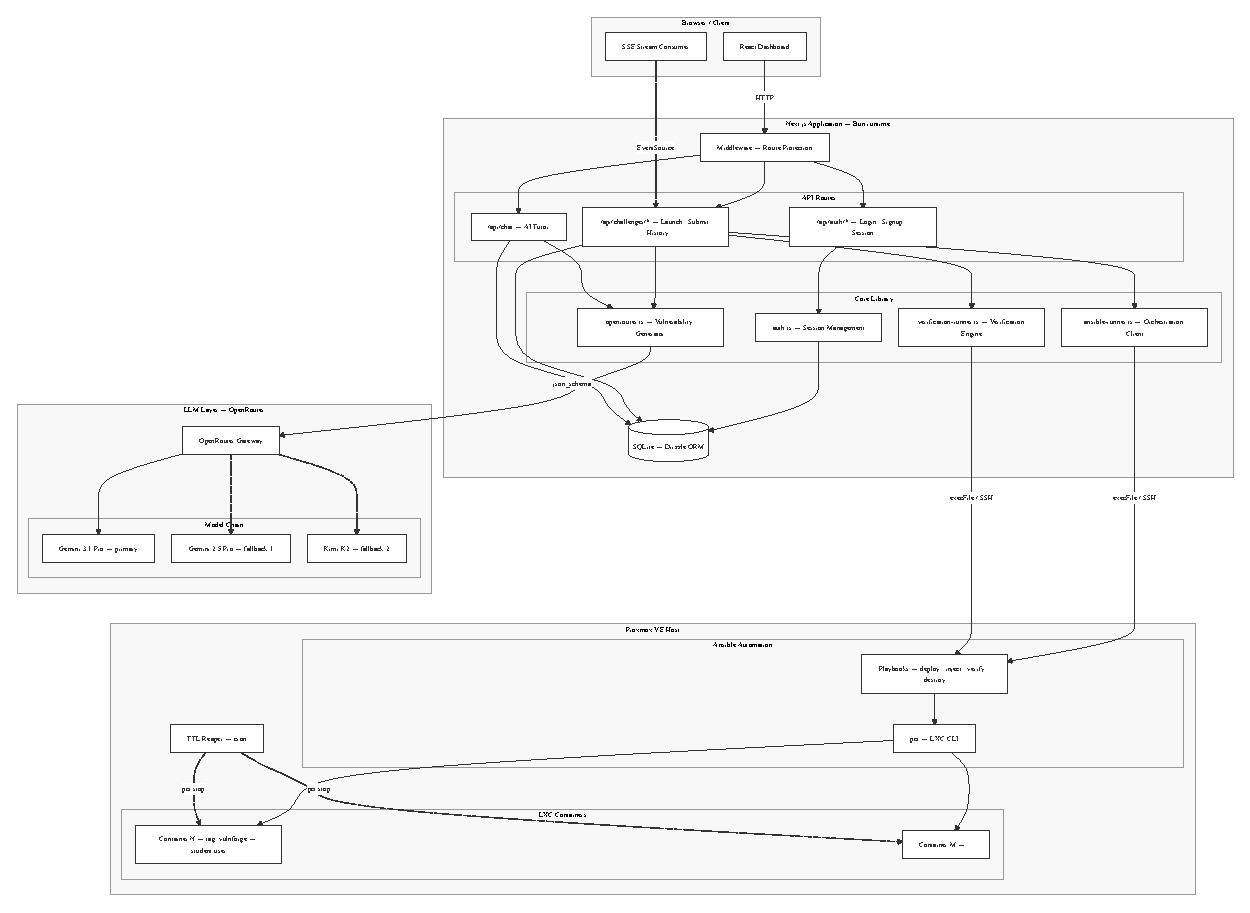
\includegraphics[
        width=\linewidth,
        height=15cm,
        keepaspectratio
    ]{mermaid/from-spec/system_architecture.pdf}
    \caption{System Architecture}
    \label{fig:system-architecture}
\end{figure}

The web application is the central part of the application. It validates user input, manages accounts and sessions, stores challenge state, invokes the LLM calls, invokes the container orchestration, presents the challenge and confirms completion. Ansible is used as the infrastructure automation layer, with Proxmox as the hypervisor. This keeps the web application focused on key operations, whilst handing over any infrastructure tasks to Ansible via Ansible Playbooks.
\marginpar{ TODO - Potentially explain what ansible \& playbooks are.}
It deliberately avoids exposing infrastructure code to users. Students do not need to interact with Proxmox, Ansible and APIs. They only interact with the generated environment and the chatbot.

\subsection{Data Model}\label{sec:data_model}

The database contains four tables: users, sessions, challenges and messages.

\begin{figure}[htbp]
    \centering
    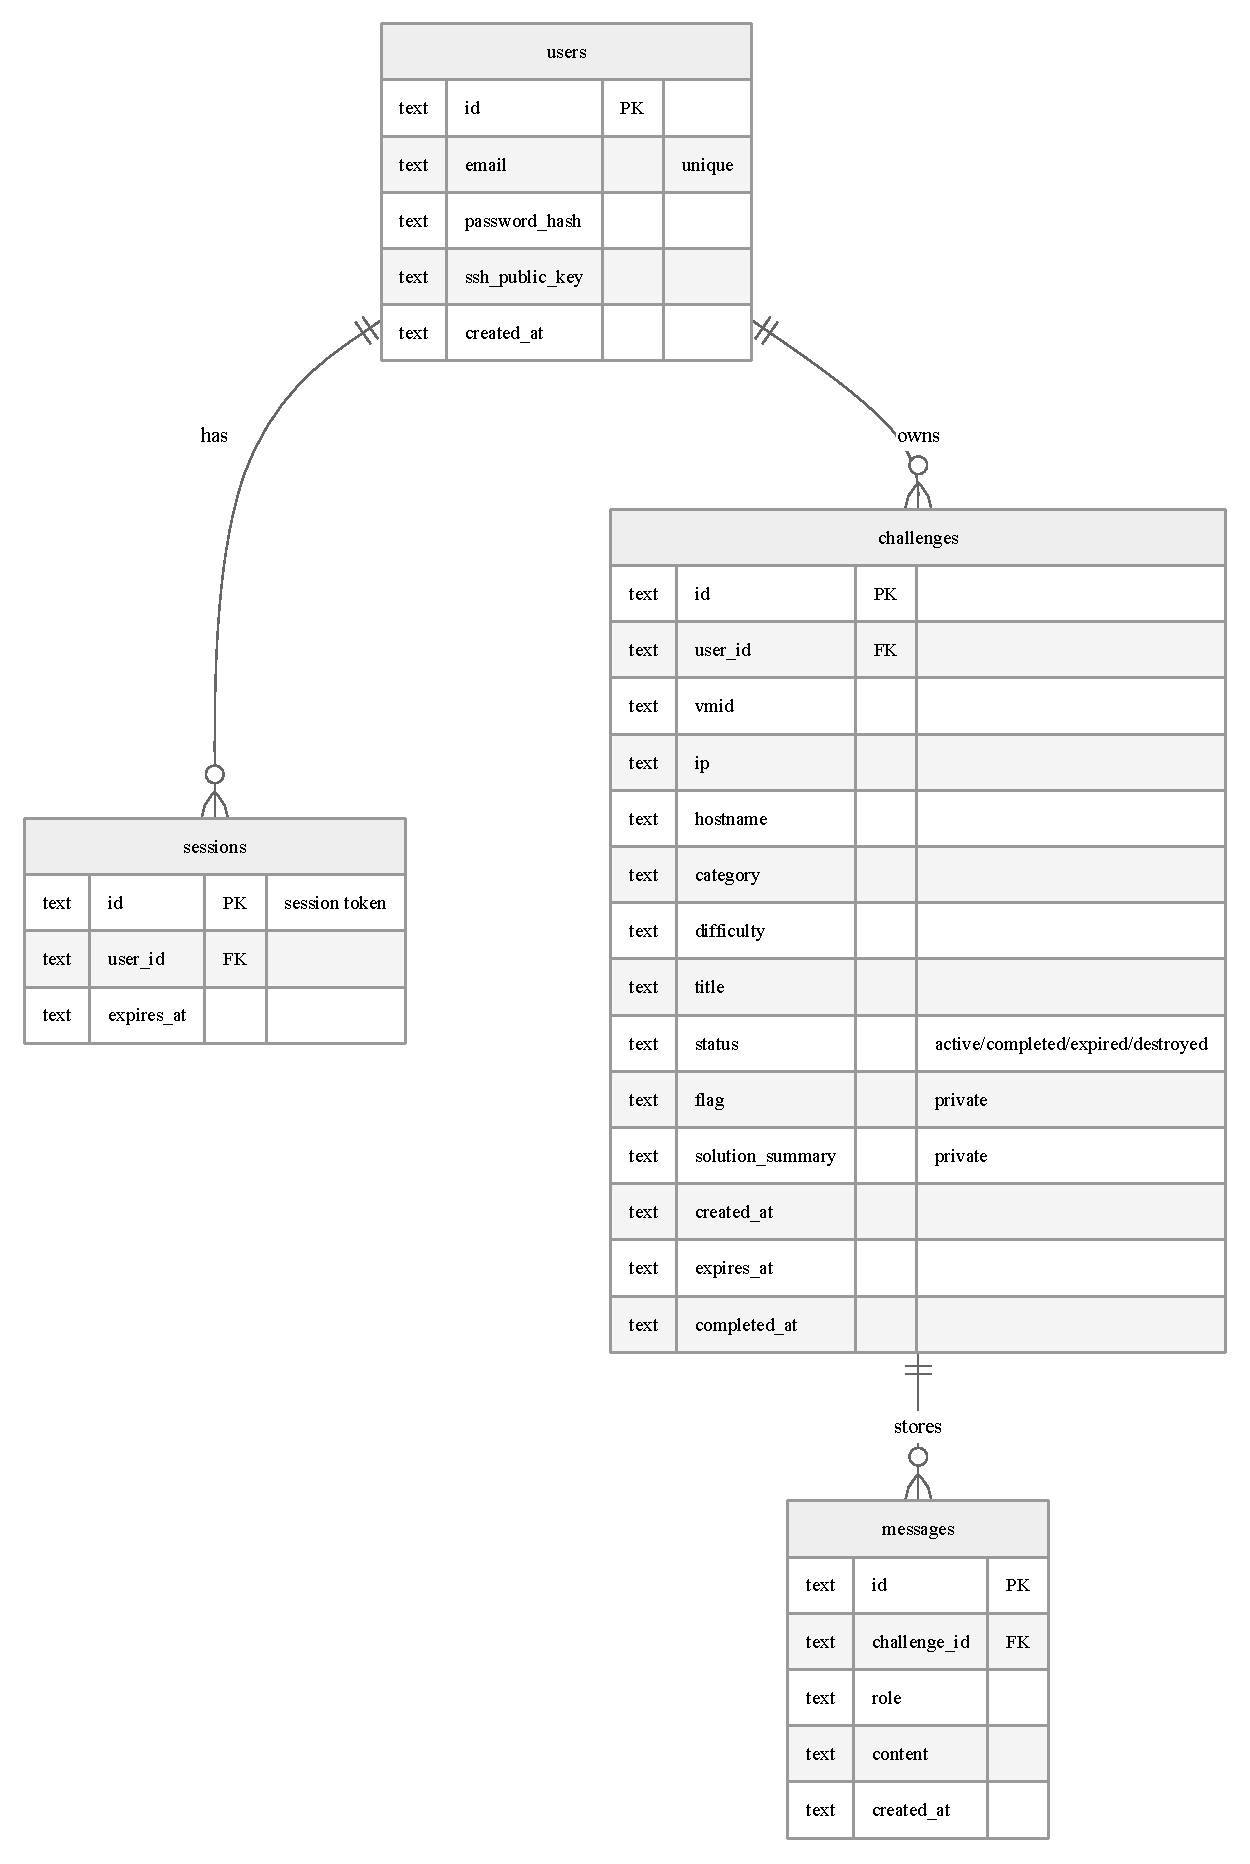
\includegraphics[
        width=\linewidth,
        height=0.82\textheight,
        keepaspectratio
    ]{figures/database_schema.pdf}
    \caption{Database schema}
    \label{fig:db_schema}
\end{figure}

The challenges table is one of the most imporatnt, connecting the user facing challenge to the generated infrastructure. It stores metadata such as title, description, hint, category, difficulty and attack vector. It also stores server only data (the flag and solution summary). Specific methods deliberately expose a public challenge type that omits these fields unless the challenge is completed, when completed, it provides the solution summary as a learning opportunity. 

The challenge is represented in four states:

\begin{table}[htbp]
    \centering
    \begin{tabular}{@{}>{\raggedright\arraybackslash}p{2cm}p{7cm}p{5cm}@{}}
        \toprule
        \textbf{Status} & \textbf{Meaning} & \textbf{Set by} \\
        \midrule
        active & The user can work on the challenge and the container is expected to exist. & Challenge creation. \\
        \addlinespace
        completed & The correct flag was submitted before expiry. & Flag submission route. \\
        \addlinespace
        destroyed & The user manually ended the challenge. & Challenge delete route. \\
        \addlinespace
        expired & The challenge exceeded its TTL. & Active challenge checks, launch cleanup, or expired flag submission handling. \\
        \bottomrule
    \end{tabular}
    \caption{Challenge status definitions}
    \label{tab:challenge-status}
\end{table}

There is a partial unique index on \lstinline|challenges(user_id)| where \lstinline|completed_as IS NULL| to enforce the idea that a user can only have one active challenge, to prevent a race condition when the same user sends multiple requests to create a challenge.

\subsection{Challenge Lifecycle}\label{sec:lifecycle}

The challenge lifecycle presented to the user is deliberatly simple, however requires careful consideration from the database and infrastructure to prevent mismatched state and inconsistencies. The application checks challenge status before chat requests, flag submissions, and deletion requests. The chat bot is only interactive in active challenges, with the history page allowing the user to view them in read-only mode. Correct flag submissions are marked as \lstinline|completed|. Manual deletion of containers marks them as \lstinline|destroyed|, and immediatgely triggers container deletion from the backend asynchronously. Expiry is handled application side, and then also by a cronjob on the host named the TTL Reaper. 

\begin{figure}[htp]
    \centering
    
\includegraphics[
        width=\linewidth,
        height=0.82\textheight,
        keepaspectratio
    ]{figures/challenge_lifecycle.pdf}
    \caption{Challenge Lifecycle}
    \label{fig:challenge_lifecycle}
\end{figure}

There is a deliberate separation between the logical flow and the infrastructure state. The database may mark a challenge as destroyed before the Ansible destroy playbook has finished running, and the TTL reaper may delete a container before the database is next checked. VulnForge accepts these possibilities as the main requirement is to prevent the user from continuing to interact with stale challenges that should be destroyed, and to prevent indefinite resource usage. Having the TTL reaper as a cronjob that runs every 5 minutes, checking container \lstinline|uptime| to see if it exceeds 60 minutes means that we can guarantee containers are cleaned up, regardless of database state. 

\subsection{Launch Pipeline}\label{sec:launch_pipeline}
The challenge launch pipeline is the most complex aspect of the project. It gets exposed to the user via the browser as a server sent event stream so that the UI can show progress as it is occuring. This is because the operations can take a while, and we do not want the user to think something has frozen, so this shows them intermediate progress. 

\begin{figure}[htbp]
    \centering
    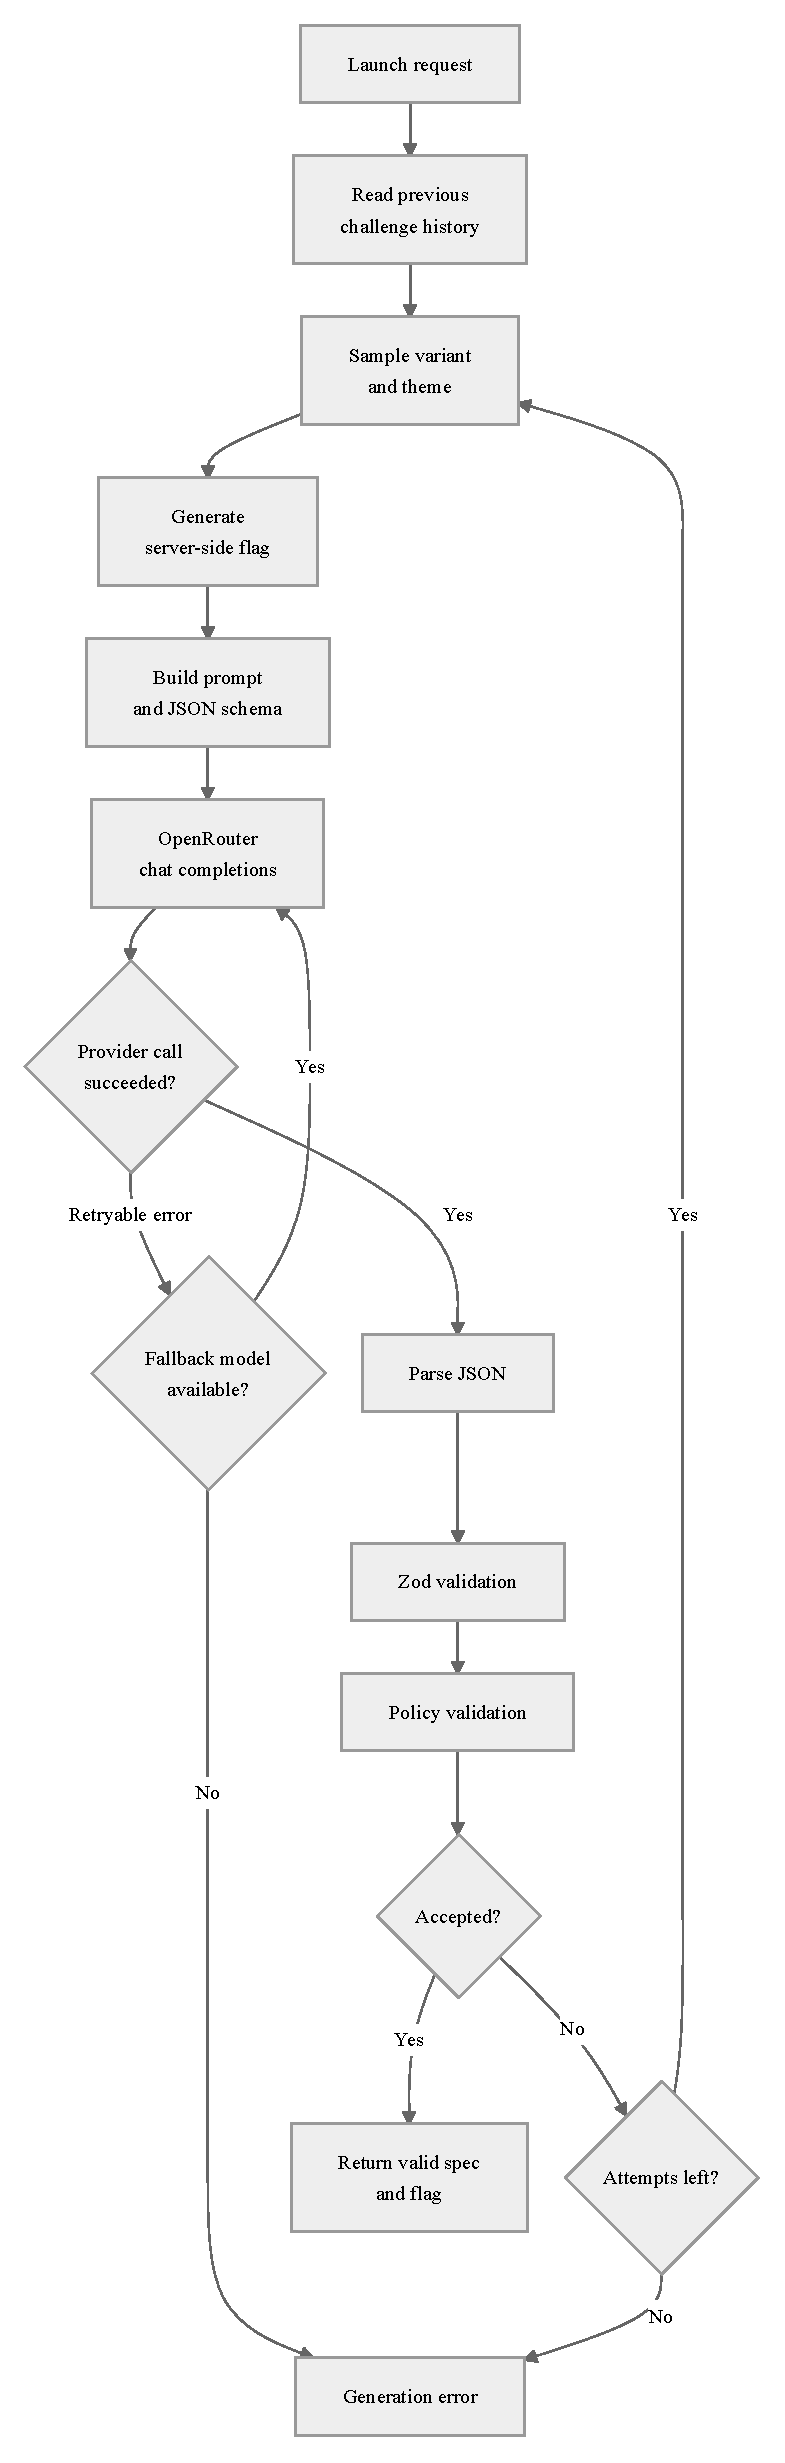
\includegraphics[
        width=\linewidth,
        height=0.82\textheight,
        keepaspectratio
    ]{figures/launch_generation.pdf}
    \caption{Launch Pipeline}
    \label{fig:launch_pipeline}
\end{figure}

The pipeline has two verification levels. Regular launches from the browser run a health verification mode. This executes health checks and flag protection checks. This can catch commonf failures such as a web server not starting, a generated file missing, or the flag being directly readable by the student. Full exploit verification is the other mode. This is controlled by an environment variable named \lstinline|CHALLENGE_FULL_VERIFY_BEFORE_LAUNCH|. When this mode is enabled, the application will first deploy a disposable container, named the 'verifier'. This container will have the generated vulnerability specfication injected into it, run the exploit checks provided by the LLM, and then if it verifies it works, destroy the temporary container and deploy a fresh user facing container. This is only used when the environment variable is enabled as it is quite time intensive, and we do not want the user to have the delay. It also avoids giving the user a container that has already been mutated by the exploit checks, as if we ran this on the users container, certain changes such as permission ones would have to be reverted, causing increased complexity. 


\subsection{Vulnerability generation design}\label{sec:vuln_gen_design}

The LLM does not directly control the infrastructure, instead it produces a structured \lstinline|VulnerabilitySpec| object that is treated as a data source. The schema includes the following:

\begin{figure}[htbp]
    \centering
    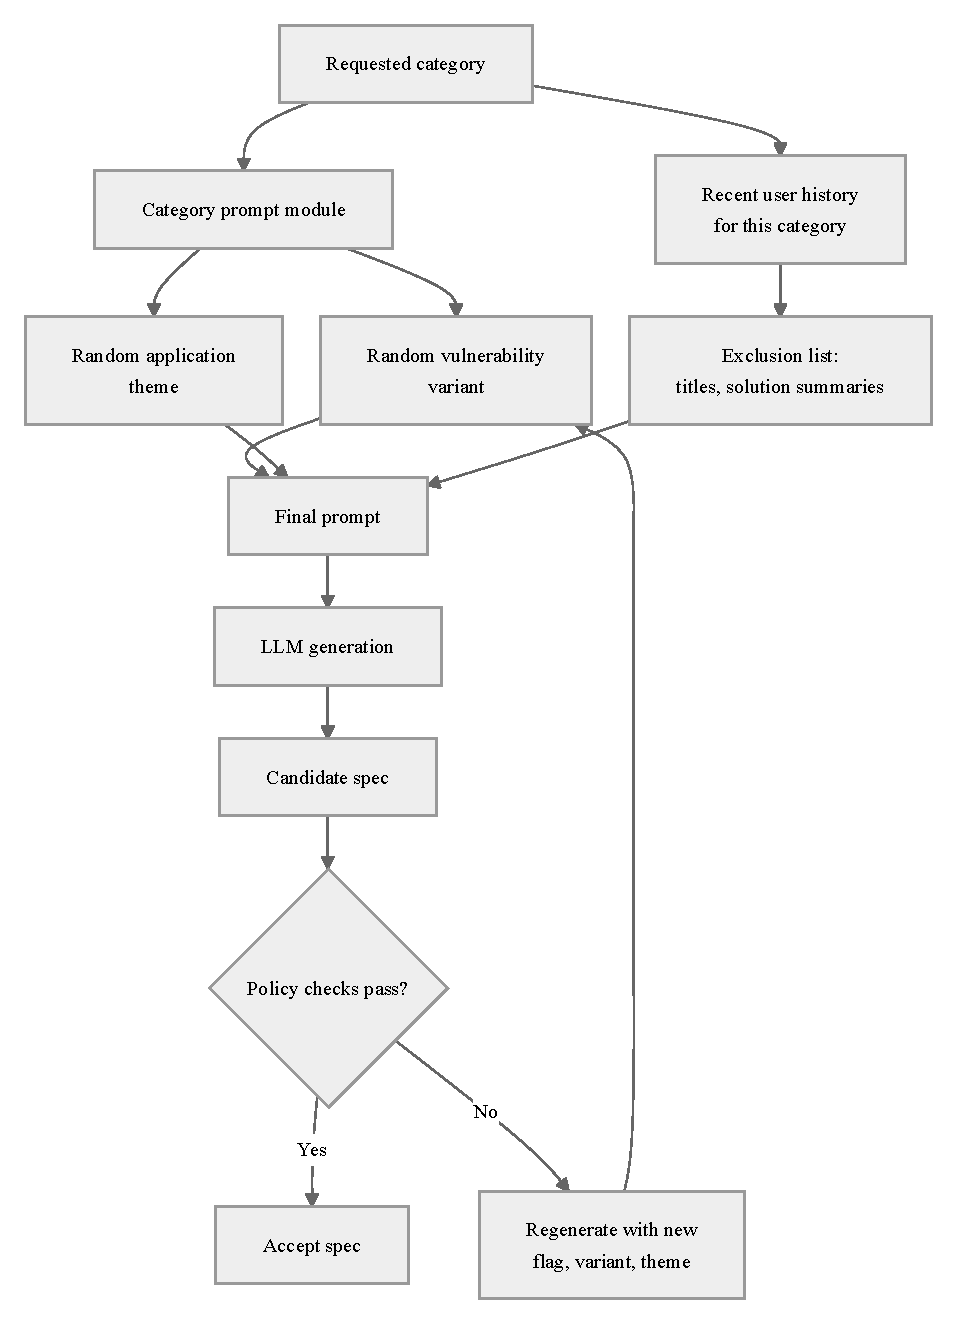
\includegraphics[
        width=\linewidth,
        height=0.82\textheight,
        keepaspectratio
    ]{figures/generation_policy.pdf}
    \caption{Generation Policy}
    \label{fig:generation_policy}
\end{figure}

The design uses various safeguards to ensure the LLM generates a vulnerability to VulnForge's specification.
\begin{enumerate}
    \item Server side flag generation: The platform generates the flag as \lstinline|FLAG{...}| using random bytes. This occurs before we call to the LLM, and the LLM is then instructed to embed this exact flag string somewhere exploitable. This avoids relying on the model to generate a unique flag, and allows us to store it in logs and context, without having to wait for the LLM call to extract it. Furthremore, any aspects we can compute server side are useful as it means that we do not need excessive LLM calls that can result in further delay. 
    \item Structured output: The Zod schema is converted to JSON, and then sent to OpenRouter. The response is still parsed, and validated again server side.
    \item Policy validation: The schema checks can verify structure, but policy validation ensures that there is not semantic issues occuring. This can include incorrect categories or difficulties, missing flags, attempts to modify \lstinline|SSH| configuration, or unsafe commands.
    \item Category specific prompts: Each vulnerability has its own prompt and variant. This prevents having one large prompt file, instead giving each category clear requirements.
    \item Diversity mechanisms: A random category is selected for each launch of a machine. Web based activities can also receive a specific application theme sucha s a booking system. Then we store the users past themes, and add them to an exclusion list, so the model does not repeat the same scenario. This is to prevent the application appearing as if it is continually generating the same scenario, providing variety to the user to keep them engaged. 
\end{enumerate}

This design allows the model to have some freedom to invent scenarios, whilst keeping them grounded in the set boundary of the rest of the system. So this way, the system interprets a typed, validated specification rather than natural language.

\subsection{Verification design}\label{sec:verification_design}

Earlier versions of the software would check just whether Ansible completed, however, we soon noticed that this was inadequate as Ansible succeeding does not necessarily mean that a usable challenge has been generated. For example, a web service may start, however, a intentional exploit path may be inaccessible. 

Each validation command contains a name, description, context, command string, timeout, expected error code, exptected stout and stderr, and a \lstinline|must_recover_flag| that can be enabled. 

\marginpar{TODO: add table}

\begin{table}[htbp]
    \centering
    \begin{tabular}{@{}>{\raggedright\arraybackslash}p{3.5cm}p{5cm}p{5cm}@{}}
        \toprule
        \textbf{Context} & \textbf{Meaning} & \textbf{Typical use} \\
        \midrule
        \lstinline{container_root} & Run inside the LXC container as root through \lstinline{pct exec}& Starting / stopping \lstinline{systemd} services and file checks\\
        \addlinespace
        completed & The correct flag was submitted before expiry. & Flag submission route. \\
        \addlinespace
        destroyed & The user manually ended the challenge. & Challenge delete route. \\
        \addlinespace
        expired & The challenge exceeded its TTL. & Active challenge checks, launch cleanup, or expired flag submission handling. \\
        \bottomrule
    \end{tabular}
    \caption{Verification Running Context}
    \label{tab:verification-runner-context}
\end{table}

The validator treats validation commands as untrusted as they are generated by the model. Host related commands such as \lstinline{pct}, \lstinline{pvesh} and \lstinline{qm} are rejected, alongside cloud metadata access, OpenRouter references, SSH commands and external HTTP checks that are not related to the target URL / container IP. This is a middle-ground we have decided on, as the model is able to describe how we should validate the specific challenge, cut the platform constraints still limit how these commands may run. 


\subsection{Tutor design}\label{sec:tutor}

The tutor is a chatbot that is aware of the context of the current challenge. When the user sends a message, the chat route loads the authenticated user's challenge, and checks the supplied challenge ID matches i. If so, it builds a system prompt containing the challenge title, description, category, difficulty, hint, attack vector and the solution summary (which is hidden from the user). 

The tutors purpose is to provide progressive guidance, it should explain concepts and suggested methods, but it should not reveal the flag or provide the entire exploit path in one response. It uses two layers of protection to enforce this:

\begin{enumerate}
    \item Firstly, the tutor has system prompt instructions, that instruct it not to reveal the flag, the flag path, or any full step-by-step solution.
    \item Secondly, the application checks the generated response response before streaming it back, and check it for a \lstinline|FLAG{...}| pattern, the stored flag, or the solution summary. If any are present, the response is replaced by a block message saying: \lstinline{"I can't provide the flag or the full exploit path. Ask for a smaller hint and I'll guide you step by step."}. The messages are persisted after each entire response by the LLM. This supports the continued educational aspect, enabling read only review in the history page to fully review how you as a user approached the challenge. 
\end{enumerate}

\subsection{Challnege history and learning review}\label{sec:challenge-history}

The history page of the application is designed to increase the educational value of the activity beyond just attacking a vulnerable machine. The history shows the entire history of challenges for the authenticated user from an internal API, containing message counts and status information.

\begin{figure}[htbp]
    \centering
    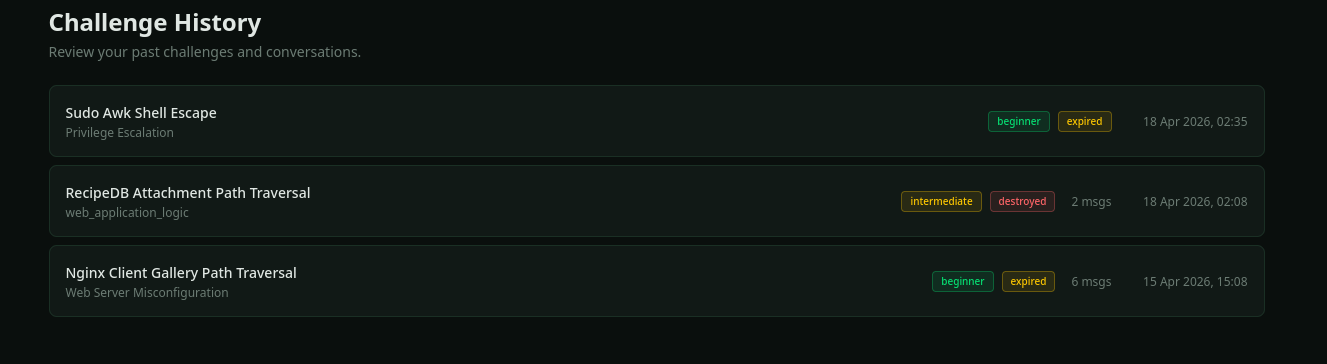
\includegraphics[
        width=\linewidth,
        height=0.82\textheight,
        keepaspectratio
    ]{images/history-overview.png}
    \caption{Overview of user history}
    \label{fig:history-overview}
\end{figure}

Then you can look at specific challenges, seeing the solution summary and your chat history to understand where you went wrong if you were unable to complete the challenge. This creates a clear distinction between the guidance offered when attempting to attack a machine, and an explanation after a successful or failed attempt. 

\begin{figure}[htbp]
    \centering
    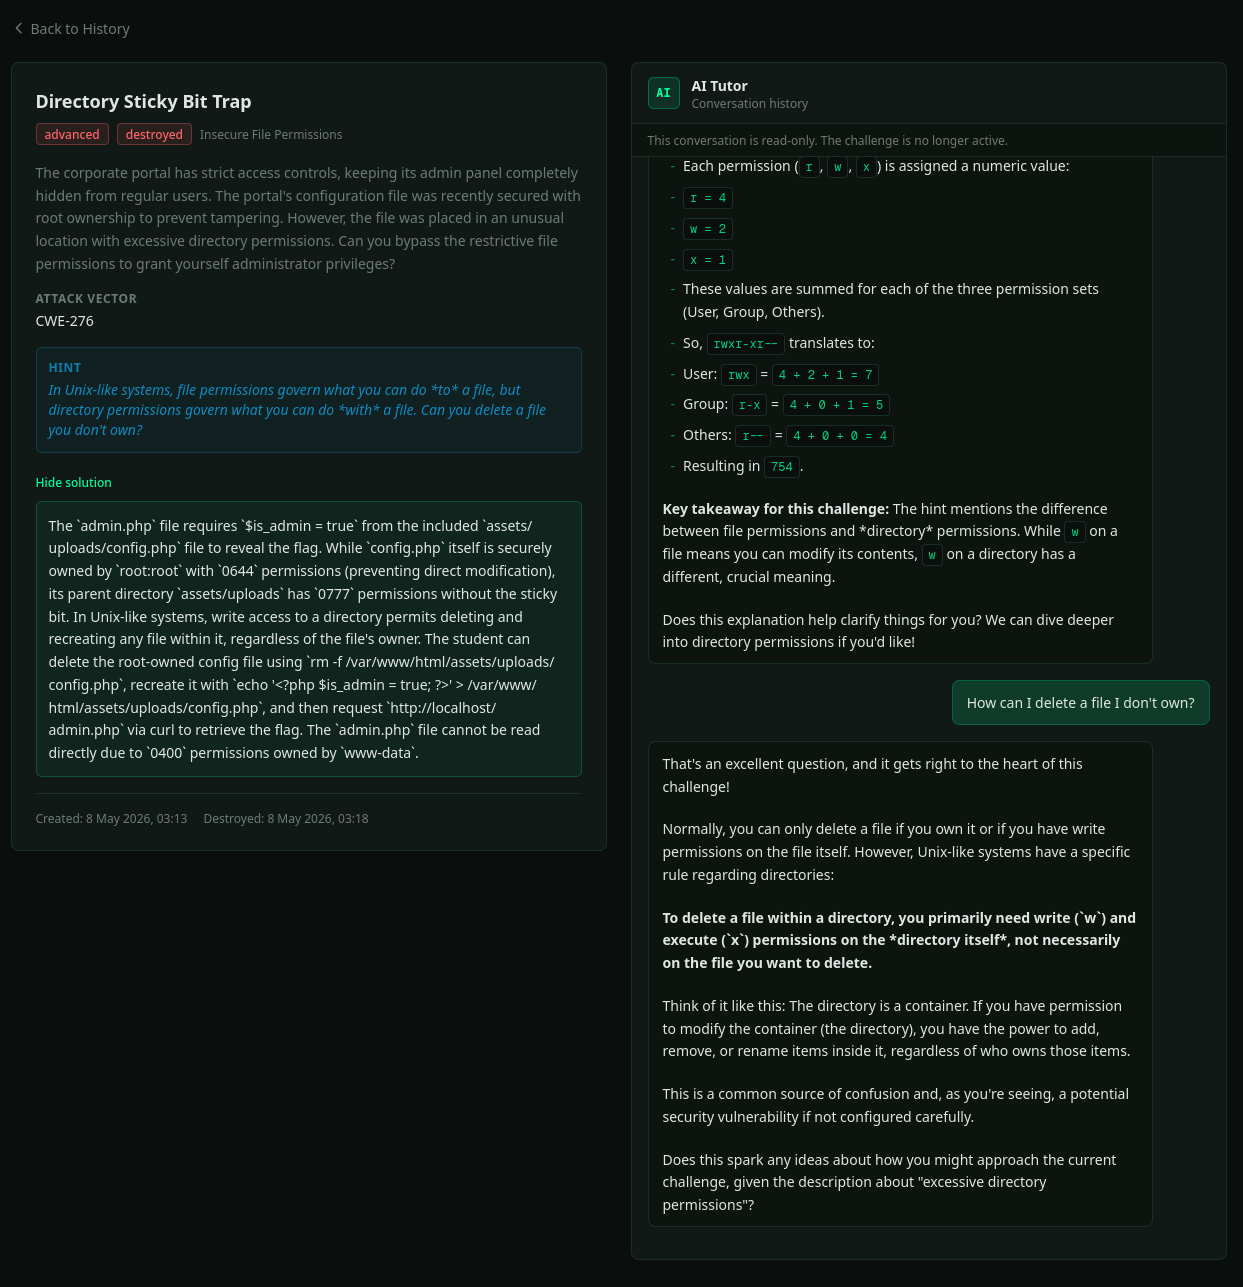
\includegraphics[
        width=\linewidth,
        height=0.82\textheight,
        keepaspectratio
    ]{images/history-challenge.png}
    \caption{History of a specific challenge}
    \label{fig:history-challenge}
\end{figure}


\section{Implementation}\label{sec:impl}

\subsection{Tech Stack \& Project Structure}\label{sec:tech-stack}

\marginpar{TODO: Add versions here}
The project was built with TypeScript and React for the web application, Drizzle ORM as a mapper for the database to allow type safe queries, SQLite as a local database, Zod for schema validation, OpenRouter for LLM integration and Pino for logging. The back end was constructed with Next.JS to have actions run on the server instead of the client, Ansible to automatically deploy and provision containers, and Proxmox as a hypervisor. 

\marginpar{TODO: add table}

Drizzle runs migrations automatically when the database is created, with SQLite being configured in WAL mode (write-ahead logging) to allow the application to perform concurrent reads and writes during actions that may have a lock on the database such as launching of challenges, or chat persistence.

\subsection{Authentication, settings and user state}\label{sec:auth-settings}

Authentication is implemented with email and password combination. Passwords are hashed with bcrypt before being stored. A successful login creates a row in the sessions table, and sets a HTTP only session cookie named \lstinline{session_token}. The cookie has a seven day expiration. API routes that require you to be logged in run \lstinline{requireAuth()} which reads the cookie from the user, check the session exists in the database and has not expired, and once these are validated, it loads the corresponding users data. 

The settings route allows the user to update their public SSH key, and password. SSH keys are validated with regular expression that accepts common SSH key types such as \lstinline{ssh-ed25519} and \lstinline{ssh-rsa}, \lstinline{ECDSA} and security key backed \lstinline{ed25519}. 
The launch route refuses to provision a new challenge if the authenticated user does not have an associated SSH key, ensuring key configuration is at the start of the workflow, displaying a message to the user saying they need to set it, this also prevents any LLM calls or container creation as we do not want extra resource usage if the user is unable to connect to the container. 

\begin{figure}[htbp]
    \centering
    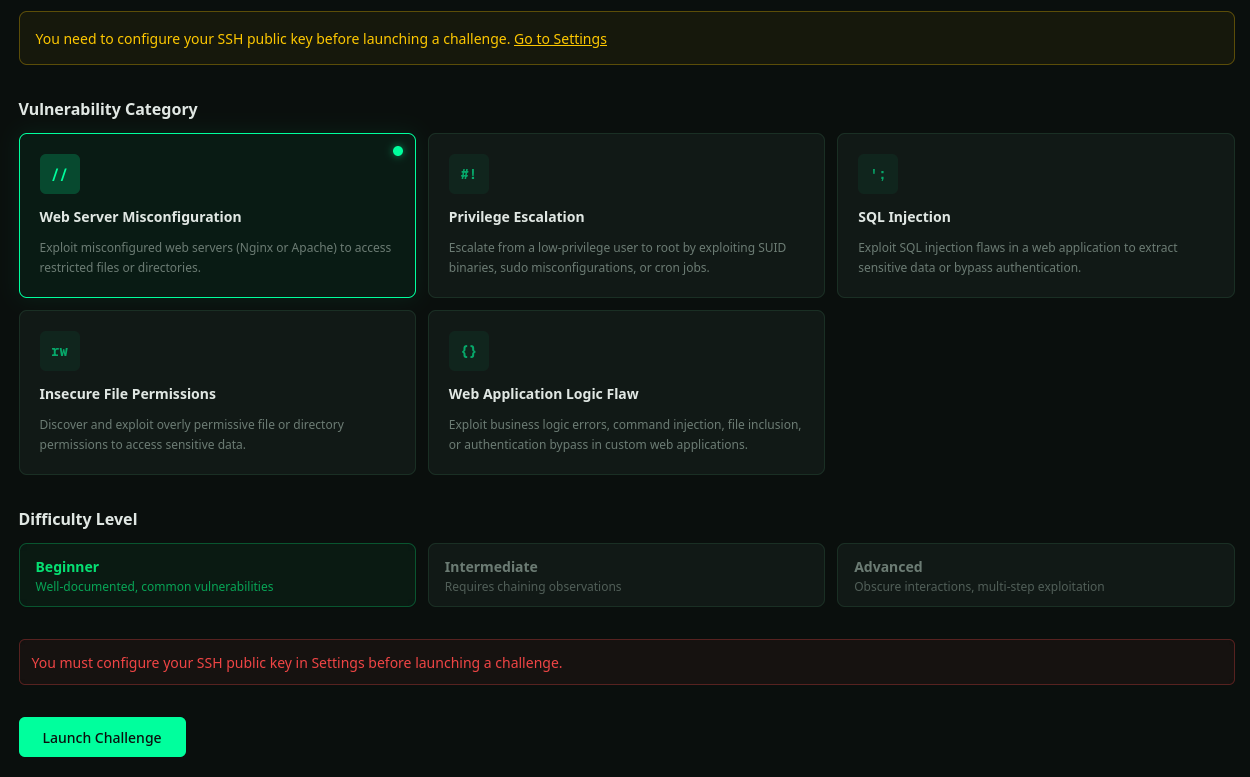
\includegraphics[
        width=\linewidth,
        height=0.82\textheight,
        keepaspectratio
    ]{images/required-ssh-key-config.png}
    \caption{User requires an SSH key before starting a challenge}
    \label{fig:ssh-key-required}
\end{figure}

\subsection{Database respositories and status transactions}\label{sec:database-reponsitories}

We have a data access layer that wraps access to any database related actions for users, sessions, challenges and messages. This prevents API routes from containing raw SQL and allows the application to have a single point to enforce domain specific behavior. Each table has its own associated respository which houses it's specific functions.


\begin{figure}[htbp]
    \centering
    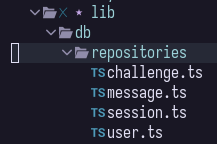
\includegraphics[
        width=\linewidth,
        height=0.82\textheight,
        keepaspectratio
    ]{images/db-repositories.png}
    \caption{Each tables database repository}
    \label{fig:db-repositories}
\end{figure}

The challenge repository creates new challenges with \lstinline{status = 'active'}, an expiry time that is one hour after creation, and a \lstinline{completed_at} timestamp. It provides methods for finding the active challenge for a user, retrieving all challenges for history, finding prior challenges from a specific category to ensure the new challenges are diverse, finding expired challenges, and transitioning a challenge from active to expired.

To enforce the rule that one user can only have one challenge we do:

\begin{enumerate}
    \item The launch route checks for an existing active challenge 
    \item The launch route re-checks before inserting into the database after we have generated a vulnerability and provisioned the machine
    \item The database has a partial unique index on active challenges for users
\end{enumerate}

The partial unique index is seen as the most important as it handles race conditions that the application may struggle to prevent. 


\subsection{OpenRouter implementation}\label{sec:openrouter-implementation}

To generate a vulnerability for a machine, the entry-point is the \lstinline{generateVulnerability()} method inside \lstinline{app/lib/openrouter.ts}. To do so, it performs the following steps:
\begin{enumerate}
    \item Generate a random flag, stored server side 
    \item Build a category specific prompt based on what the user has selected, the difficulty, the random variant and theme (based on the users history) - this is classed as the user prompt
    \item Convert the Zod internal schema into a JSON schema that the LLM can adhere to 
    \item Send the system prompt, alongside the user propmt to OpenRouter with the structured response format 
    \item Parse the returned text as JSON 
    \item Validate it against the internal \lstinline{VulnerabilitySpecSchema}
    \item Run semantic validation
\end{enumerate}

\begin{center}
\begin{minipage}{\linewidth}
\captionsetup{type=listing,hypcap=false}
\caption{\texttt{VulnerabilitySpecSchema} that the LLM should adhere to}
\label{code:VulnerabilitySpecSchema}
\end{minipage}
\end{center}
\begin{minted}{TypeScript}
    export const ValidationSpecSchema = z.object({
  health_checks: z.array(ValidationCommandSchema).min(1),
  flag_protection_checks: z.array(ValidationCommandSchema).min(1),
  exploit_checks: z.array(ValidationCommandSchema).min(1),
});

/**
 * The complete vulnerability specification returned by OpenRouter
 * We view it as the contract between the LLM and the injection pipeline
 */
export const VulnerabilitySpecSchema = z.object({
  title: z
    .string()
    .describe(
      "A short, human-readable title for this vulnerability scenario, e.g. 'Nginx Path Traversal via Misconfigured Alias'"
    ),
  description: z
    .string()
    .describe(
      "A 2-4 sentence description of the vulnerability, what it is, and why it is dangerous. This will be shown to the user as their briefing."
    ),
  category: z
    .string()
    .describe(
      "The vulnerability category, e.g. web_server_misconfiguration, privilege_escalation, sql_injection"
    ),
  difficulty: z
    .enum(["beginner", "intermediate", "advanced"])
    .describe("The intended difficulty level of this challenge"),
  hint: z
    .string()
    .describe(
      "A single cryptic hint that nudges the user toward the attack vector without revealing the solution"
    ),
  apt_packages: z
    .array(AptPackageSchema)
    .describe(
      "List of apt packages that must be installed for the vulnerable service to function"
    ),
  files: z
    .array(FileEntrySchema)
    .min(1)
    .describe(
      "The files to write into the container. Must include all configuration, application code, and the flag file."
    ),
  services: z
    .array(ServiceSchema)
    .describe(
      "Systemd services to restart or enable after files are injected"
    ),
  setup_commands: z
    .array(z.string())
    .default([])
    .describe(
      "Optional shell commands to run inside the container after file injection and service restart, for any setup that cannot be expressed as files (e.g. creating database tables, adding system users). Each command is run as root via pct exec."
    ),
  solution_summary: z
    .string()
    .describe(
      "A concise explanation of how to exploit this vulnerability and retrieve the flag. This is stored server-side and NEVER shown to the user; it is used by the tutor LLM to provide contextual hints."
    ),
  attack_vector: z
    .string()
    .describe(
      "The MITRE ATT&CK technique or CWE identifier most relevant to this vulnerability, e.g. CWE-22 (Path Traversal) or T1059 (Command and Scripting Interpreter)"
    ),
  validation: ValidationSpecSchema.describe(
    "Private server-side validation commands used to verify the challenge before presentation and during evaluation. Must include at least one health check, one flag-protection check, and one exploit check. Never shown to the student."
  ),
});
\end{minted}

\subsection{Prompt catalogue and diversity implementation}\label{sec:prompt-catalogue}

Initially, to generate a vulnerability, we had just one prompt file, but as we expanded the variation of vulnerabilities, we realised that this needed to be segmented more, so it developed into a catalogue of category modules that are selected based on the users selection. Currently we support the following categories:

\begin{enumerate}
    \item Web Server Misconfiguration
    \item Privilege Escalation
    \item SQL Injection
    \item Insecure File Permissions
    \item Web Application Logic Flaws
\end{enumerate}

Each category has a user facing label and description of what it entails, then behind the scenes, there is a list of variants, and themes (where supported) and a prompt template. The prompt builder chooses a random variant, and for web categories, it chosses a random theme. This helps ensure that two identical requests for the same vulnerability and difficulty should not produce the same style of vulnerability. 

The prompt builder is also able to query previous challenges for the user to ensure they do not get the same category. It goes through the recent titles and solution summaries, and passes them into the prompt as part of an exclusion list, which the LLM is instructured not to use so a user would not get the same vulnerability and scenario twice. The evaluation harness which runs after the vulnerability is created measures the diversity in a more concrete way, using generated titlesl, attack vectors and file hashes to further ensure that the vulnerability is different. 

\subsection{Container deployment}\label{sec:container-deployment}
 
Container deployment is implemented through the \lstinline{deploy.yml} playbook and the \lstinline{lxc_lifecycle.yml} role. The playbook creates an Ubuntu 24.04 unprivileged LXC container with one core, 1024 MB of memory, 8 GB root filesystem, DHCP on the \lstinline{vmbr0} interface and the \lstinline{vulnforge} tag inside Proxmox. It then starts the container, creates the \lstinline{student} user, injects the user's SSH key, waits to be assinged an IP address, then writes to a deployment artefact that containers the VMID, hostname, IP address and configuration details. 


\begin{center}
\begin{minipage}{\linewidth}
\captionsetup{type=listing,hypcap=false}
\caption{\texttt{Deployment Artefact}}
\label{code:deployment-artefact}
\end{minipage}
\end{center}
\begin{minted}{JSON}
{
    "cores": 1,
    "created_at": "2026-04-16T14:43:24.435859",
    "hostname": "lab-1776346995",
    "ip": "192.168.0.81",
    "memory": 1024,
    "net0": "name=eth0,bridge=vmbr0,ip=dhcp",
    "rootfs": "local-lvm:8",
    "template_file": "ubuntu-24.04-standard_24.04-2_amd64.tar.zst",
    "vmid": "112"
}
\end{minted}

\section{Summary}\label{sec:summary}
% Optional: short summary of the methodology. Omit if the chapter is already conciseq
